\section{Dise\~no de funciones transferencias con RLC ideal}




\subsection{High-pass y low-pass}

Los filtros se implementan con circuitos RLC serie. Para el low-pass la salida se toma en el capacitor, y para el high-pass, en el inductor. Se obtienen las siguientes funciones transferencia:\\

\begin{description}%sym tf de HP y LP
	
	\item[\textbf{Low-pass}]
	
	\begin{equation}
	\frac{1}{\left(\frac{s}{2\pi f_{0LP}}\right)^2 + \frac{s}{2\pi f_{0LP}} \cdot 2\xi + 1}
	\label{eq:ej2_LP_tf_syms}
	\end{equation}	
	
	\item[\textbf{High-pass}]
	
	\begin{equation}
	\frac{\left(\frac{s}{2\pi f_{0HP}}\right)^2}{\left(\frac{s}{2\pi f_{0HP}}\right)^2 + \frac{s}{\omega _0}\cdot 2 \xi + 1}
	\label{eq:ej2_HP_tf_syms}
	\end{equation}

\end{description}


\subsection{Relaci\'on entre filtro low-pass y high-pass}

\todo{mejorar el flujo de ideas de esta secci\'on porque es media una verga}

\begin{itemize}	%simetria plantilla HP LP y cambio de variable

	\item Como se observa en la tabla \ref{tab:ej2_plantilla}, las plantillas de los filtros high-pass y low-pass presentan una s\'imetr\'ia: la frecuencia de paso ($f_p$) de uno es la frecuencia de atenuaci\'on ($f_a$) del otro, y la atenuaci\'on en $f_a$ es igual para ambos filtros (\'idem con $f_p$). 
	
	\item Siempre que la frecuencia sea analizada en escala logar\'itmica, la respuesta en frecuencia de un filtro high-pass de orden 2 tiene la forma de un filtro low-pass de orden 2 pero espejado sobre un eje vertical. Esto permite obtener la respuesta en frecuencia de un filtro high-pass de orden 2 a partir de la de un filtro low-pass de orden 2. Se detalla un ejemplo en la figura \ref{fig:ej2_LP2HP_example}. Cabe destacar que los cambios de variables para pasar de una funci\'on transferencia a otra no modifican el $\xi$ del sistema.

\end{itemize}

Teniendo en cuenta los dos puntos anteriores, se dise\~na la transferencia del low-pass y se la espeja en la media logar\'itmica 
\footnote{Se utiliza la media logar\'itimica y no la lineal ya que la simetr\'ia existe siempre que se analice a la frecuencia en escala logar\'itmica, no lineal.} 
$f_{med\, log}  = \sqrt{f_a f_p} \approx 7.5KHz$ para obtener la del high-pass.


\begin{figure*}	%LP2HP_ejemplo
	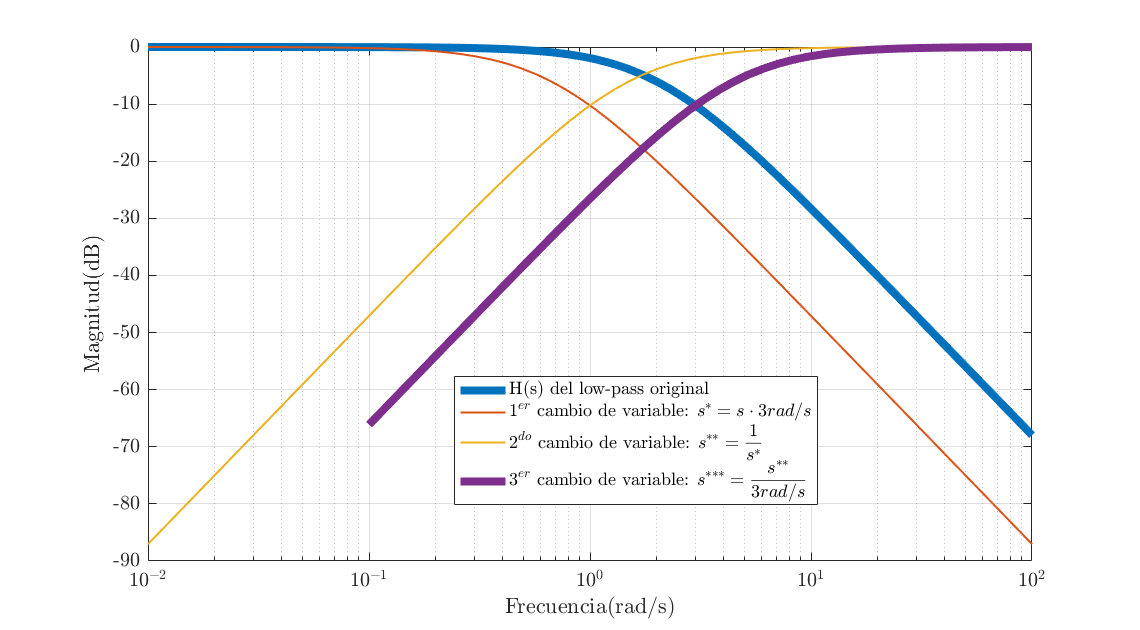
\includegraphics[width = \textwidth]{imagenes/LP2HP_example.png}
	\caption[Trasformaci\'on de filtro low-pass a high-pass]{Trasformaci\'on de filtro low-pass a high-pass mediante inversi\'on en el eje de $3\, rad/s$. El primer cambio de variable mueve la transferencia de forma que el punto que estaba en $3\, rad/s$ se desplace hasta $1\, rad/s$ . El segundo espeja respecto el eje de $1\, rad/s$, y el tercero desplaza nuevamente a $3\, rad/s$. La funcion transferencia inicial es $H_{LP}(s) = \frac{1}{\frac{s^2}{4}+s+1}$, y la final $H_{HP}(s) = \frac{s^2\cdot \frac{4}{81}}{s^2\cdot \frac{4}{81}+s\cdot \frac{4}{9}+1}$. Notar que las frecuencias de corte ($2\, rad/s$ para el low-pass y $4.5\, rad/s$ para el high-pass) tambi\'en se espejan respecto al eje de $3\, rad/s$ y que $\xi=1$ no se modifica.}
	\label{fig:ej2_LP2HP_example}
\end{figure*}


 



\subsection{Low-pass}

De la secci\'on \ref{ssec:ej2_H_rlc_ideal} se obtiene la transferencia de un pasabajos $RLC$ serie:

	\begin{equation}
	\frac{1}{\left(\frac{s}{2\pi f_{0LP}}\right)^2 + \frac{s}{2\pi f_{0LP}} \cdot 2\xi + 1}
	\label{eq:ej2_LP_tf_syms}
	\end{equation}	
	

Se verifica que una transferencia $f_{0\,LP}=f_{med\, log}$ cumple con la plantilla si $\xi = 1$\footnote{Solo hay sobrepico si $\xi\leqslant \frac{1}{\sqrt{2}}\approx 0.707$}. Se eligen estos valores ya que al realizar la transformaci\'on de low-pass a high-pass se cumple que 
\begin{equation}
	f_{med\, log} = f_{0LP} = f_{0HP}
	\label{eq:ej2_f0_LP_HP}
\end{equation} 
Esto presenta ventajas a la hora de elegir valores de componentes (ver secci\'on \ref{ssec:ej2_HP_componentes}).


\begin{align}	%xi=>alfa,^L=>R
	\alpha &= \frac{R}{2L}	\\
	\intertext{Como $\xi = 1 \Rightarrow \alpha = \omega _0$:}
	2\pi f_0 &= \frac{R}{2L}\\ 
	R &= 2\pi f_0 \cdot 2L 	\\
	&= 1.88K\Omega			\\
	\intertext{Ajustando a valores comerciales:}
	R &= 1.8K\Omega
\end{align}

\begin{align}	%w0^L=>C
	\omega_0 &= \frac{1}{\sqrt{LC}}		\\
	C &= \frac{1}{L\cdot (2\pi f_0)^2}	\\
	&= 22.5nF 							\\
	\intertext{Ajustando a valores comerciales:}
	C&=22nF
\end{align}

Una vez obtenidos los valores de los componentes, se puede concluir los valores reales de $\xi$ y $f_0$:

\[\xi = \frac{R}{2} \sqrt{\frac{C}{L}} = \frac{1.8K\Omega}{2} \cdot \sqrt{\frac{22nF}{0.02H}}=0.9439 \]
\[f_0 = \frac{1}{\sqrt{LC}} = \frac{1}{\sqrt{0.02H\cdot 22nF} }\approx47.7K\Omega\]

\subsection{High-pass}	\label{ssec:ej2_HP_componentes}

\begin{align}	%f0HP = f0LP => CHP = CLP ^ LHP = LLP
f_{0\, HP} &= f_{0\, LP} \\
\frac{1}{\sqrt{L_{LP}C_{LP}}} &= \frac{1}{\sqrt{L_{HP}C_{HP}}}
\end{align} 

De acuerdo al criterio de dise\~no de reducir los diferentes valores de componentes, se elige que $C_{HP} = C_{LP}$ y $L_{HP} = L_{LP}$.
Como adem\'as la transformaci\'on no modifica el $\xi$ del filtro, 

\begin{align} %xiHP = xiLP => RHP = RLP
\xi_{LP} &= \xi_{HP}	\\
\frac{\alpha_{LP}}{2\pi f_{0\, LP}}&=\frac{\alpha_{HP}}{2\pi f_{0\, HP}} \\
\alpha_{LP} &= \alpha_{HP} \\
\frac{R_{LP}}{2L_{LP}} &= \frac{R_{HP}}{2L_{HP}} \\
R_{LP} &= R_{HP}
\end{align}

\subsection{Band-reject}

El filtro band-reject se implementa con un circuito RLC serie tomando la salida en el capacitor e inductor. Tiene la siguiente funcion transferencia:

\begin{equation}
	\frac{\left(\frac{s}{\omega _0}\right)^2+1}{\left(\frac{s}{\omega _0}\right)^2+\left(\frac{s}{\omega _0}\right)\cdot 2\xi +1}
	\label{eq:ej2_BR_tf_syms}
\end{equation}

Sabiendo que $f_{c} = 4K\Omega$, es evidente que no se pueden mantener los valores de $C$ y de $L$ usados en los filtros low-pass y high-pass
ya que tienen otra frecuencia de corte. Se elige cambiar la frecuencia de corte modificando el valor de $C$ y no de $L$ ya que de esta forma se puede usar el mismo dise\~no de gyrator.

\begin{equation}
	C = \frac{1}{L \omega_0^2} = \frac{1}{0.02H\cdot (2\pi 4KHz)^2} = 79nF \approx 82nF
	\label{eq:ej2_BR_C}
\end{equation}

en donde en el \'ultimo t\'ermino se ajust\'o a valores comerciales. Con esta aproximaci\'on se obtiene la frecuencia de corte real:

\begin{equation}
	f_{cBR} = \frac{1}{\sqrt{LC}\cdot 2\pi} = \frac{1}{\sqrt{0.02H\cdot 82nF}\cdot 2\pi} \approx 3.93KHz 
	\label{eq:ej2_BR_f0}
\end{equation}

Se elige mantener el valor de la resistencia del low-pass y high-pass ($R=1.8K\Omega$). Con todos los componentes elegidos, se obtiene el $\xi$ del circuito:
\begin{equation}
	\xi = \frac{\alpha}{\omega_0} = \frac{R}{2}\cdot \sqrt{\frac{C}{L}} = 1.8223
	\label{eq:ej2_BR_xi}
\end{equation}

Tambi\'en se puede obtener $Q=\frac{1}{2\xi}$

\begin{equation}
	Q = \frac{1}{2\xi} = 0.2743
	\label{eq:ej2_BR_xi}
\end{equation}


\subsection{Band-pass}
Dado que todos los filtros usan el mismo dise\~no de gyrator, se mantiene el valor de $L=0.02H$. Sabiendo que $f_0=8KHz$:

\begin{align*}
2\pi &= \frac{1}{\sqrt{LC}} \\
C &= \frac{1}{0.02H (2\pi 8KHz)^2} = 19.8nF\\
\intertext{Ajustando a valores comerciales:}
C &= 22nF
\end{align*}

Se decide aproximar a $22nF$ y no a $18nF$ ya que ambos valores presentaban una diferencia del mismo orden, y el primero era el mismo que fue asignado a $C$ en dos de los otros tres filtros.

Al igual que en el filtro band-reject, se mantiene el valor de $R=1.8K\Omega$

\section{Adaptaci\'on de las funciones transferencia a RLC con bobina con resistencia en serie $R_L$}

ME DA TODO CASI IGUAL SI $R_L = 50\Omega$
